%% V1.0
%% by Gabriel Garcia, gabrcg@gmail.com
%% This is a template for Udacity projects using IEEEtran.cls

%% Be Udacious!

\documentclass[10pt,journal,compsoc]{IEEEtran}

\usepackage[pdftex]{graphicx}
\usepackage{cite}
\hyphenation{op-tical net-works semi-conduc-tor}


\begin{document}

\title{Deep RL Arm Manipulation}

\author{Seyfi Gozubuyuk}

\markboth{DEEP RL, Robotics Nanodegree Program, Udacity}%
{}
\IEEEtitleabstractindextext{%

\begin{abstract}
In this project, the aim is to create a DQN agent and define reward functions to teach a robotic arm to touch the object. The project uses jetson-utils and jetson-reinforcement libraries and the Gazebo simulation environment.
\end{abstract}

% Note that keywords are not normally used for peerreview papers.
\begin{IEEEkeywords}
Robot, IEEEtran, Udacity, \LaTeX, Reinforcement Learning, RL, DEEP RL, DQN, jetson.
\end{IEEEkeywords}}


\maketitle
\IEEEdisplaynontitleabstractindextext
\IEEEpeerreviewmaketitle
\section{Introduction}
\label{sec:introduction}

\IEEEPARstart{T}{he} problem is to train a DQN agent to enable a robotic arm to do the following tasks
\begin{enumerate}
  \item Touch the object with any part of the robot arm, with 90\% accuracy.
  \item Touch the object with the gripper base of the robot arm, with 80\%accuracy.
\end{enumerate}

The jetson jetson-utils and jetson-reinforcement libraries are used to realize this project\cite{git:jtsnrl}. The Gazebo is the simulation environment for the robotic arm. There is a tube object, and the robot should learn to reach to this object.\\
The project defines several reward functions and tunes the parameters of the libraries.

\section{Background}
The problem is to build a QDN agent. The agent uses image data and reward values as input and outputs the action best action to perform.

\subsection{Reinforcement Learning}
In reinforcement learning (RL), the software agents learn the best actions in an environment to maximize the reward. The rewards should be defined for the agents. They start learning with trial and error. As they learn, they can take logical actions\cite{wiki:rl}.

\subsection{Q-learning}
In Q-learning, the agent learns a policy which contains best actions in the different states of the environment \cite{wiki:ql}. It is a model-free algorithm and does not need to know the every detail of the environment. It aims to build a table to store rewards for each state and action pair. At every time step, the agent observes it state and choose an action. Then it updates the reward value of that state, action pair.

\subsection{Deep Reinforcement Learning}
Deep reinforcement learning (DRL) is a special kind of reinforcement learning that uses artificial neural networks to train the agent. It replaces the processing sensor measurements step with an end-to-end approach. The network directly receive the sensor measurements and returns the best action to perform\cite{wiki:drl}.

\subsection{Deep Q Network}
DQN trains an NN for the Q value function. It uses the following techniques to let the network converge faster and more reliably.

\begin{itemize}
\item The replay pool takes the average of the behavior distribution over previous states. It is essential for smoothing the learning and handling the noise. It provides the advantage of using every step more than once in the weight update process.
\item The target network represents the Q function that is the function to compare when calculating the loss. Since the Q function values are changing during the training, it is required to use another network.
\end{itemize}

\section{Simulations}
The simulation environment is in Gazebo. There exist two nodes. The camera node and the collision node. The agent should subscribe to the topics of these nodes. The agent is an instance of the dqnAgent provided by the jetson-reinforcement library.\\
There were two options for controlling the arm joints. The first one is the velocity control. In the beginning, it was the preferred approach; however, the agent using this approach was not successful. One issue with this controller is, it requires an additional action for not changing any velocities. The other method was the position control. This approach directly changes the position of the joint.\\
There are three rewards in general. They can be listed as follows.
\begin{itemize}
\item Reward for the successful end of episode
\item Reward for the unsuccessful end of episode
   \begin{itemize}
     \item Hit to the ground
     \item End of episode without success
     \item Touch the object with other parts than gripper (Only for task 2)
   \end{itemize}
\item Reward Delta, based on distance for each episode.
\end{itemize}
There are two parameters for these rewards. They are REWARD\textunderscore WIN and REWARD\textunderscore LOSS, and they were set to 100 and -100 respectively, in order to increase the difference between the end of episode rewards and episode rewards. However, there are multipliers for these parameters.\\
There are five different distance functions. The first one existed in both tasks, but the others were explored in the second task. The first function, BoxDistance, calculates the distance between the nearest points of two boxes, the gripper and the tube.\\
The hyperparameters used in both tasks are given in Table~\ref{table:params}. Since the hardware that the project run on has limited resources, it was required to decrease the complexity of the neural network.
\begin{table}[h]
\caption{Hyperparameters}
\label{table:params}
\begin{center}
\begin{tabular}{|c||c||c|}
\hline
Parameter & Task 1 & Task2\\
\hline
INPUT\textunderscore WIDTH &   64 & 64 \\
\hline
INPUT\textunderscore HEIGHT &  64 & 64 \\
\hline
OPTIMIZER & RMSprop & RMSprop \\
\hline
LEARNING\textunderscore RATE & 0.05 & 0.02 \\
\hline
REPLAY\textunderscore MEMORY & 10000 & 10000 \\
\hline
BATCH\textunderscore SIZE & 8 & 16 \\
\hline
USE\textunderscore LSTM & true & true \\
\hline
LSTM\textunderscore SIZE & 16 & 16 \\
\hline
\end{tabular}
\end{center}
\end{table}


\subsection{Task 1}
The reward for the successful end of episode was set 2 times REWARD\textunderscore WIN minus the episodeFrames property of the ArmPlugin class. The reason was to produce a value which was always higher than the REWARD\textunderscore WIN parameter and to penalize the increasing number of steps.\\
The reward for hit the ground and episode exceeds the maximum number of frames had the value of the REWARD\textunderscore LOSS parameter. This were good enough to penalize the end of episode without success.\\
The distance reward that was calculated in each episode had the value of the REWARD\textunderscore WIN parameter multiplied by the moving average of the delta of the distance to the goal. The other parameter was the alpha which was equal to 0.25. The reason for keeping alpha small is to increase the effect of the last delta values.


\subsection{Task 2}
The robot arm from the previous task only aimed to touch the tube no matter which part reaches before. The first thing to try was adding a penalty for robot parts other than the gripper touches the object. However, this does not help the agent to change its behavior. Therefore, this project investigated several reward functions.\\
The changes applied to the reward functions are as follows.
\begin{itemize}
\item Reward for the successful end of episode
   \begin{itemize}
     \item Collision with arm gripper middle had a reward multiplier of 16 (16 * REWARD\textunderscore WIN - episodeFrames)
     \item Collision with arm gripper base had a reward multiplier of 8 (8 * REWARD\textunderscore WIN - episodeFrames)
   \end{itemize}
\item Reward for the unsuccessful end of episode
   \begin{itemize}
     \item Hit to the ground has a multiplier 1.8 (1.8 * REWARD\textunderscore LOSS)
     \item End of episode without success (REWARD\textunderscore LOSS)
     \item Touch the object with other parts than gripper (REWARD\textunderscore LOSS)
   \end{itemize}
\item Reward based on distance for each episode.
   \begin{itemize}
     \item Reward Delta from the previous task divided by 2
     \item Add a negative reward of Manhattan distance between the centers of two boxes
     \item Add the distance between min z of the gripper and the ground
   \end{itemize}
\end{itemize}
The success rewards were increased to encourage the robot to learn the task. Since it was better to touch the object with the gripper middle, it has a higher multiplier. And it was still important to reach the goal in early steps.\\
The penalty for hitting the ground was increased because the robot was inclined to touch the ground with the gripper before moving forward on the x-axis. Raising the threshold caused the robot to move along the x-axis without turning the joint 2. The Reward Delta was causing the same problem; therefore, it was divided with 2.\\
There was a need for other rewards changing on each frame because the end of episode rewards were not adequate. One of the additional rewards had the value of the distance between the gripper and the tube. This distance was between the centers of the boxes, and it was a Manhattan distance. It has no multipliers. The other reward was based on the minimum z value of the gripper. It was added as a reward if the gripper intersects the hyperplane of the tube extended along the z-axis. Otherwise, as a penalty, if the gripper is close to the ground. If either min.x or max.x value of the gripper was between min.x and max.x of the tube, and the same applied for the y-axis, then the gripper was assumed to intersect the hyperplane. In this case, the REWARD\textunderscore WIN divided by the minimum z value of the gripper to achieve the reward value. Otherwise, the minimum z value was compared with eight times the ground contact value. In other words, if the minimum z value was less than 0.4, a penalty was added in the same manner.\\
During the second task, additional cost functions were created. These are as follows.
\begin{itemize}
\item Manhattan distance version of the box distance
\item Center distance, finds the centers of the boxes and calculates the euclidean distance between them
\item Manhattan distance version of the center distance
\item Hit distance, calculates the nearest Manhattan distance for collision assuming the robot will reach from the upper left corner of the tube.
\end{itemize}

\section{Results}
The ArmPlugin.cpp file was able to utilize the jetson-reinforcement framework and to teach a robot arm to successfully reach the object. The previous sections describe the reward functions, hyperparameters and this section includes the results and screenshots.
\subsection{Task 1}
Figures~\ref{fig:t1s841},~\ref{fig:t1s842},~\ref{fig:t1s991}, and ~\ref{fig:t1s992} shows the screenshots of a successful run for Task 1.
\begin{figure}[thpb]
      \centering
      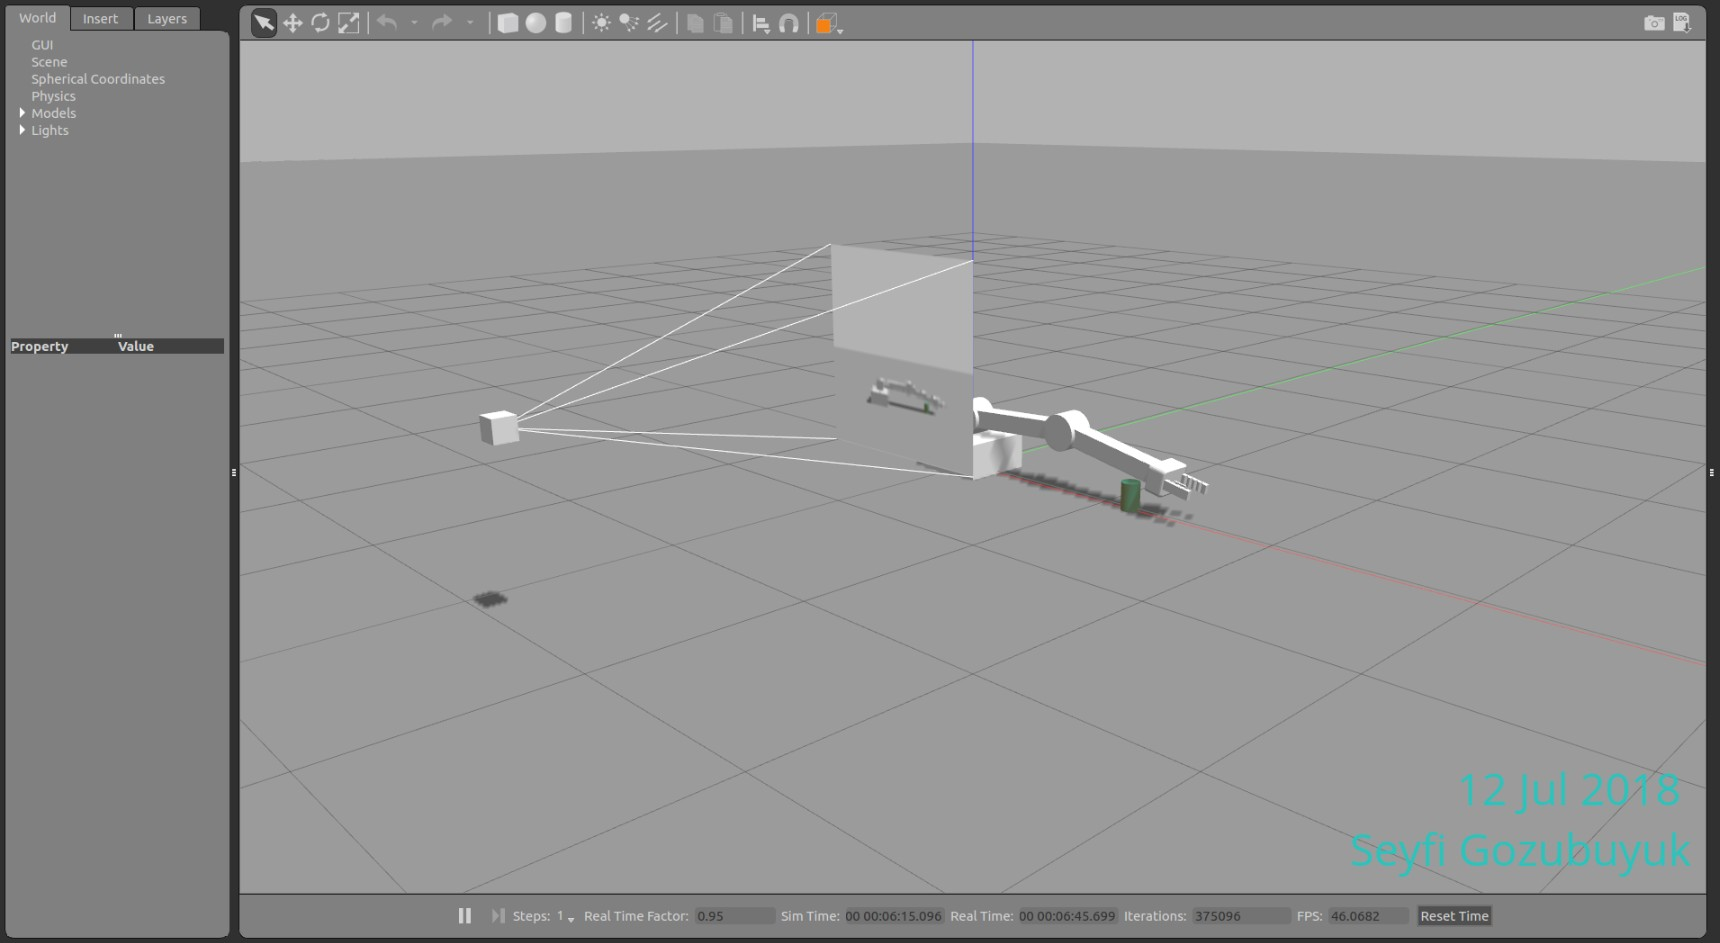
\includegraphics[width=\linewidth]{figures/Task1_Step84_1.png}
      \caption{Task 1 Episode 84 Gazebo}
      \label{fig:t1s841}
\end{figure}

\begin{figure}[thpb]
      \centering
      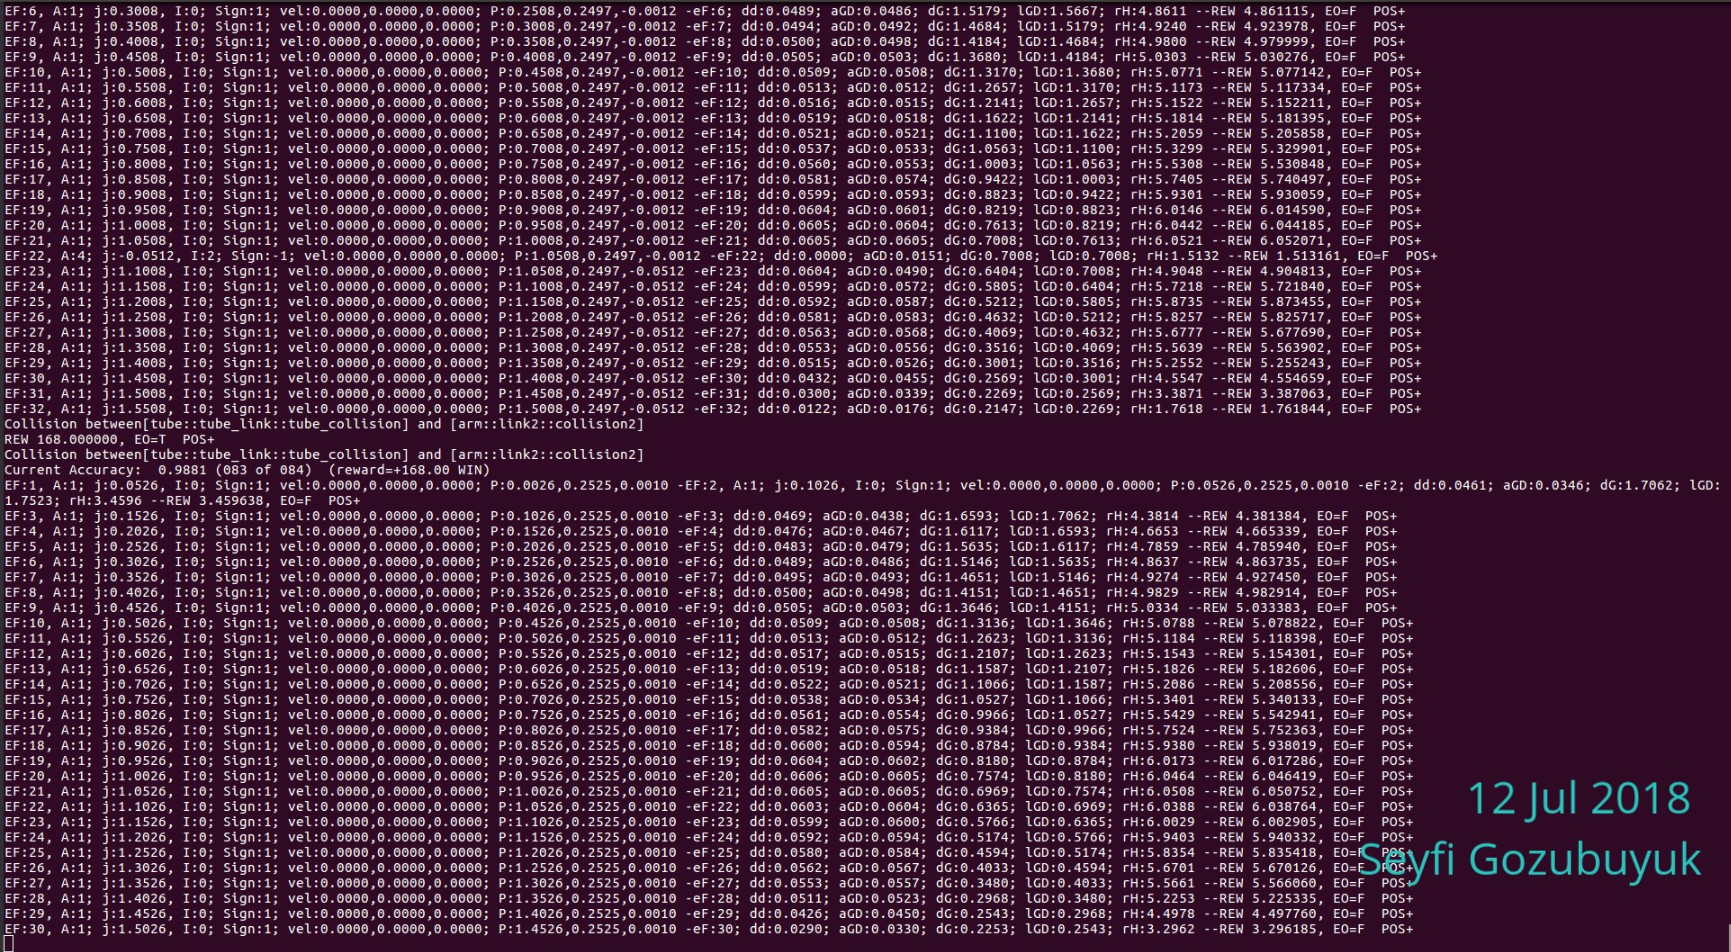
\includegraphics[width=\linewidth]{figures/Task1_Step84_2.png}
      \caption{Task 1 Episode 84 Console}
      \label{fig:t1s842}
\end{figure}

\begin{figure}[thpb]
      \centering
      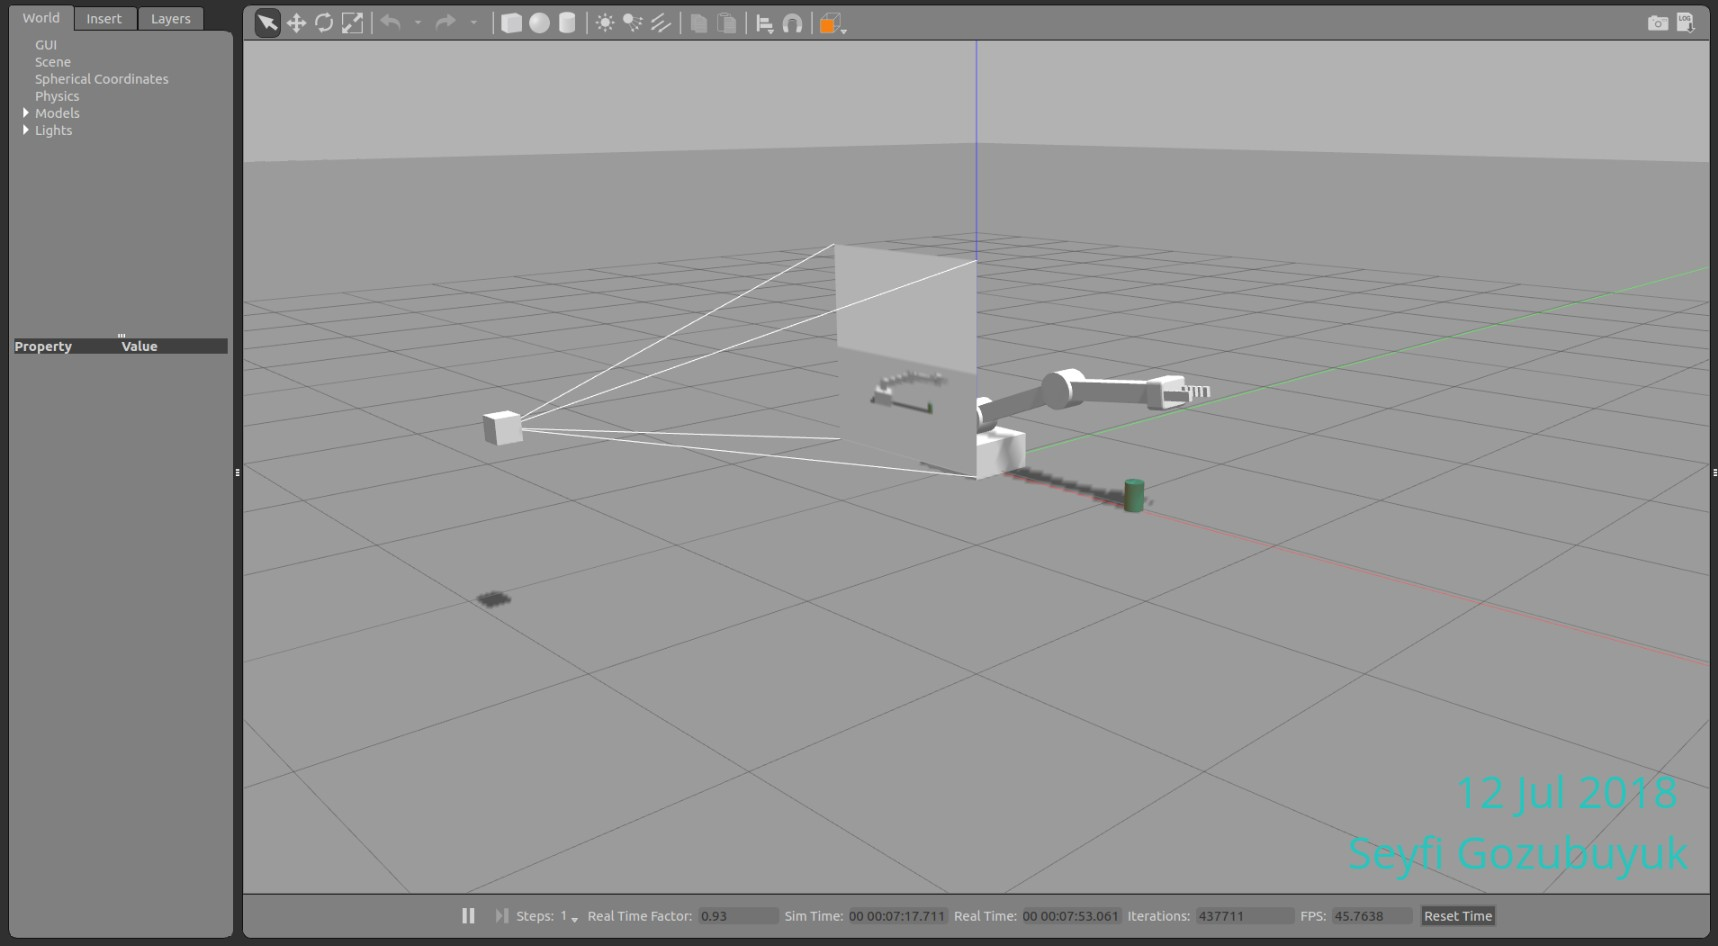
\includegraphics[width=\linewidth]{figures/Task1_Step99_1.png}
      \caption{Task 1 Episode 99 Gazebo}
      \label{fig:t1s991}
\end{figure}

\begin{figure}[thpb]
      \centering
      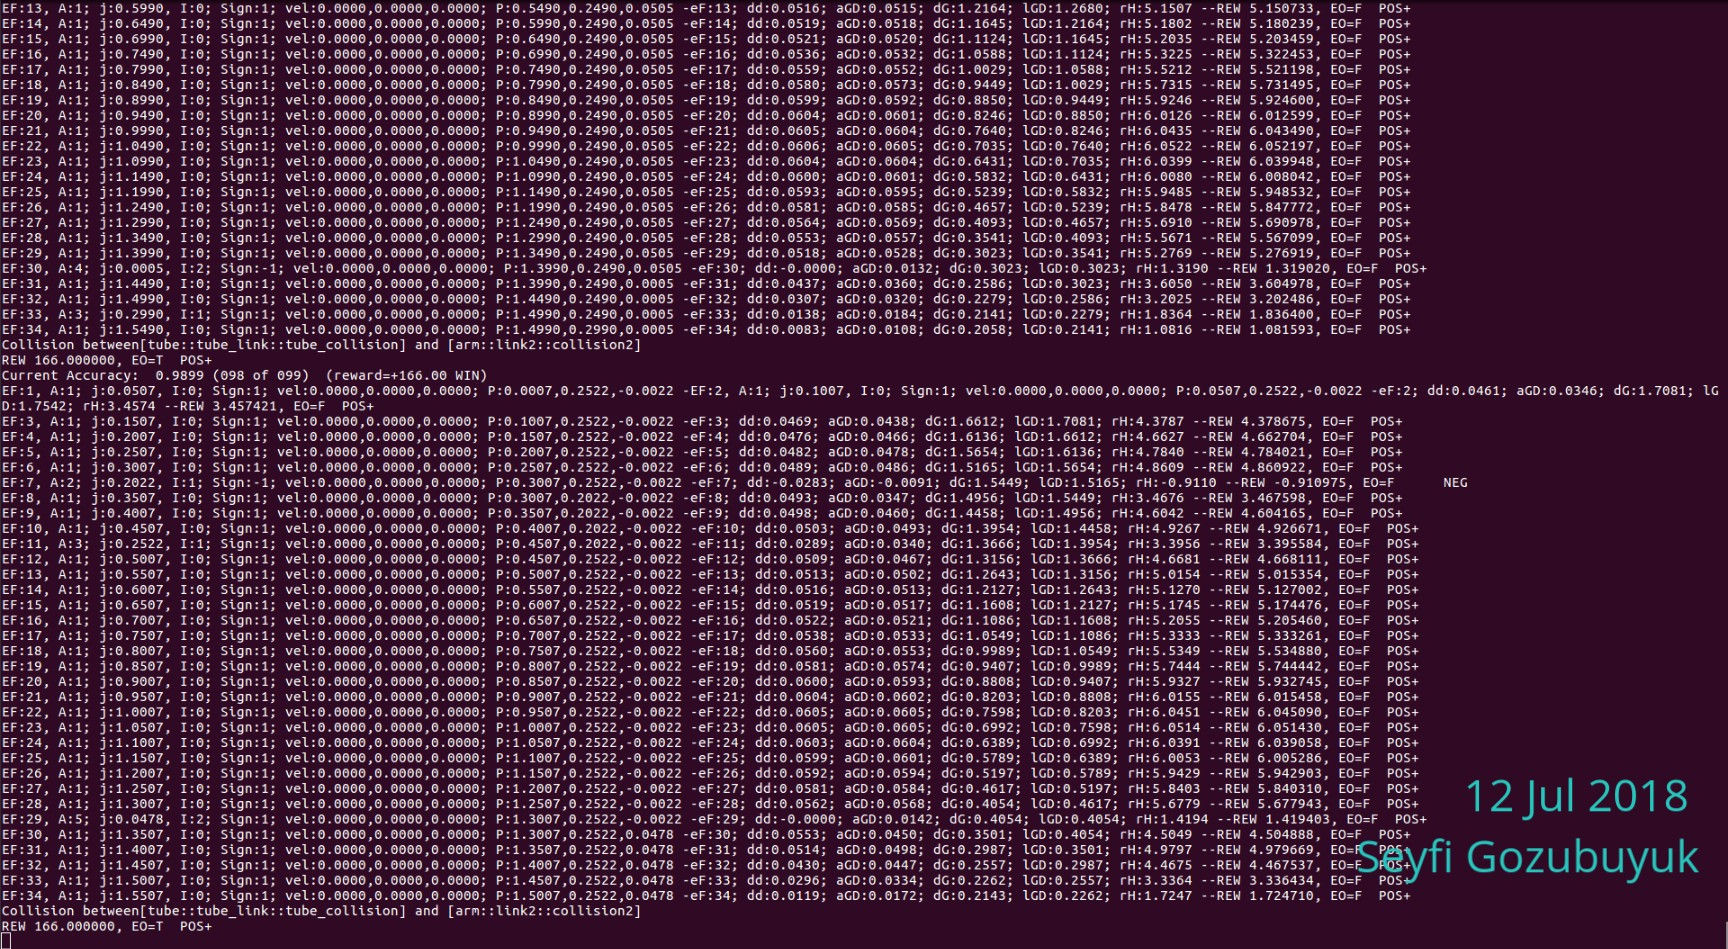
\includegraphics[width=\linewidth]{figures/Task1_Step99_2.png}
      \caption{Task 1 Episode 99 Console}
      \label{fig:t1s992}
\end{figure}
\subsection{Task 2}
Figures~\ref{fig:t2s551},~\ref{fig:t2s552},~\ref{fig:t2s941},~\ref{fig:t2s942},~\ref{fig:t2s1131}, and ~\ref{fig:t2s1132} shows the screenshots of a successful run for Task 1.
\begin{figure}[thpb]
      \centering
      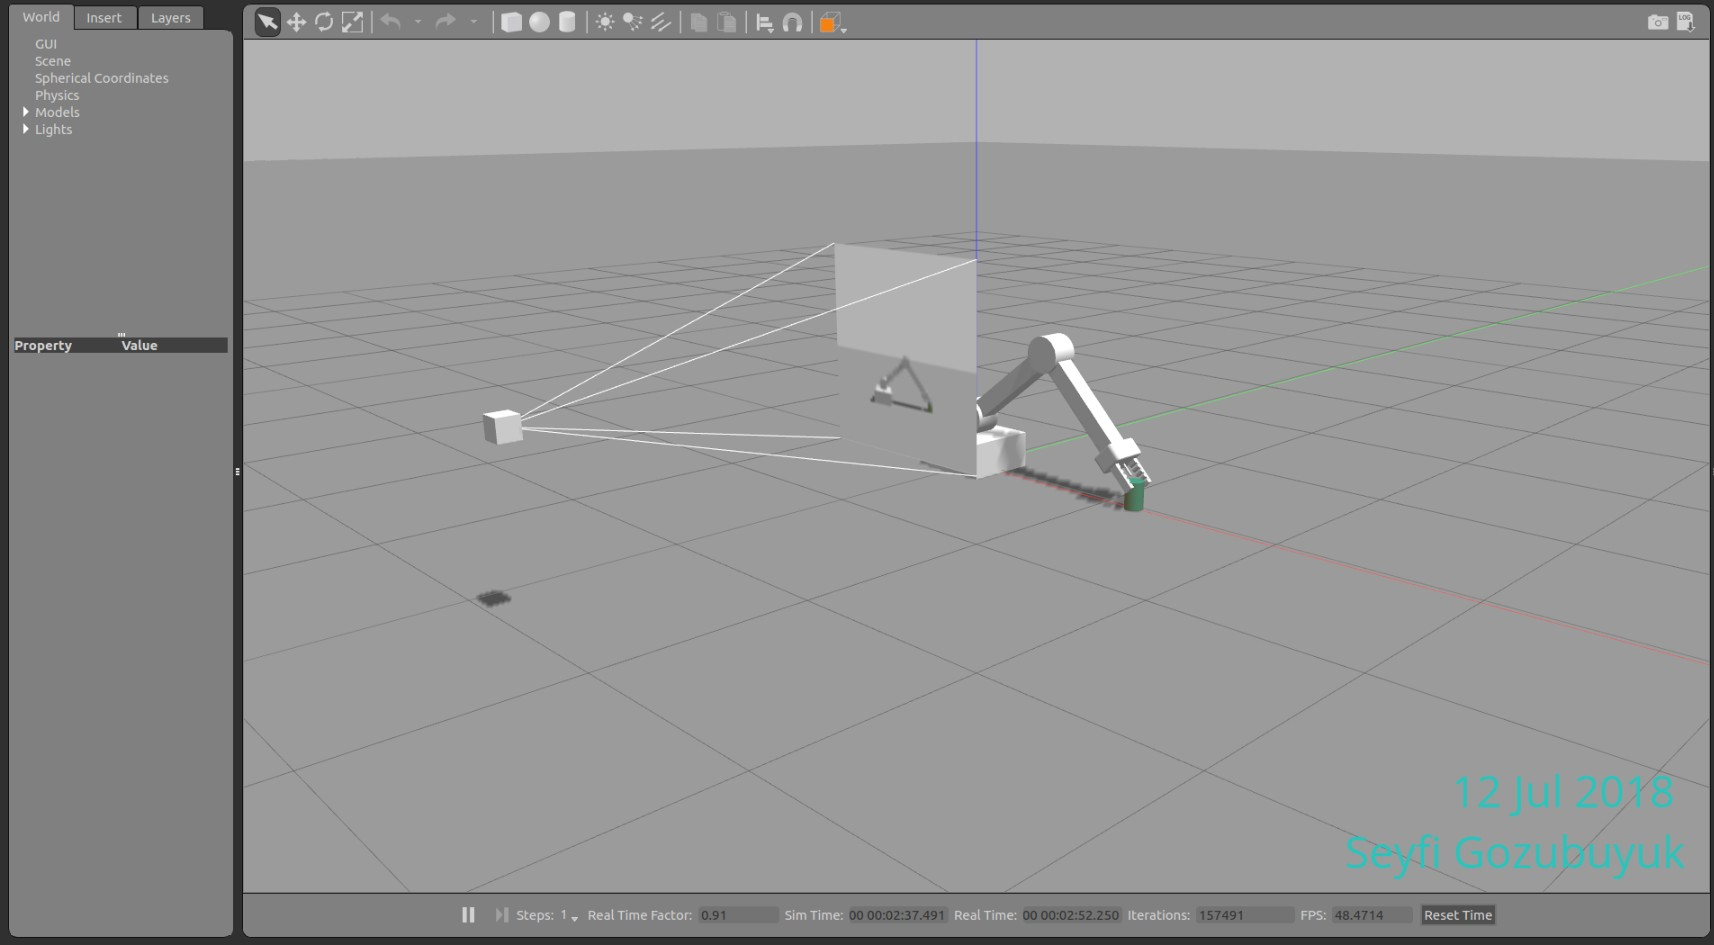
\includegraphics[width=\linewidth]{figures/Task2_Step55_1.png}
      \caption{Task 2 Episode 55 Gazebo}
      \label{fig:t2s551}
\end{figure}

\begin{figure}[thpb]
      \centering
      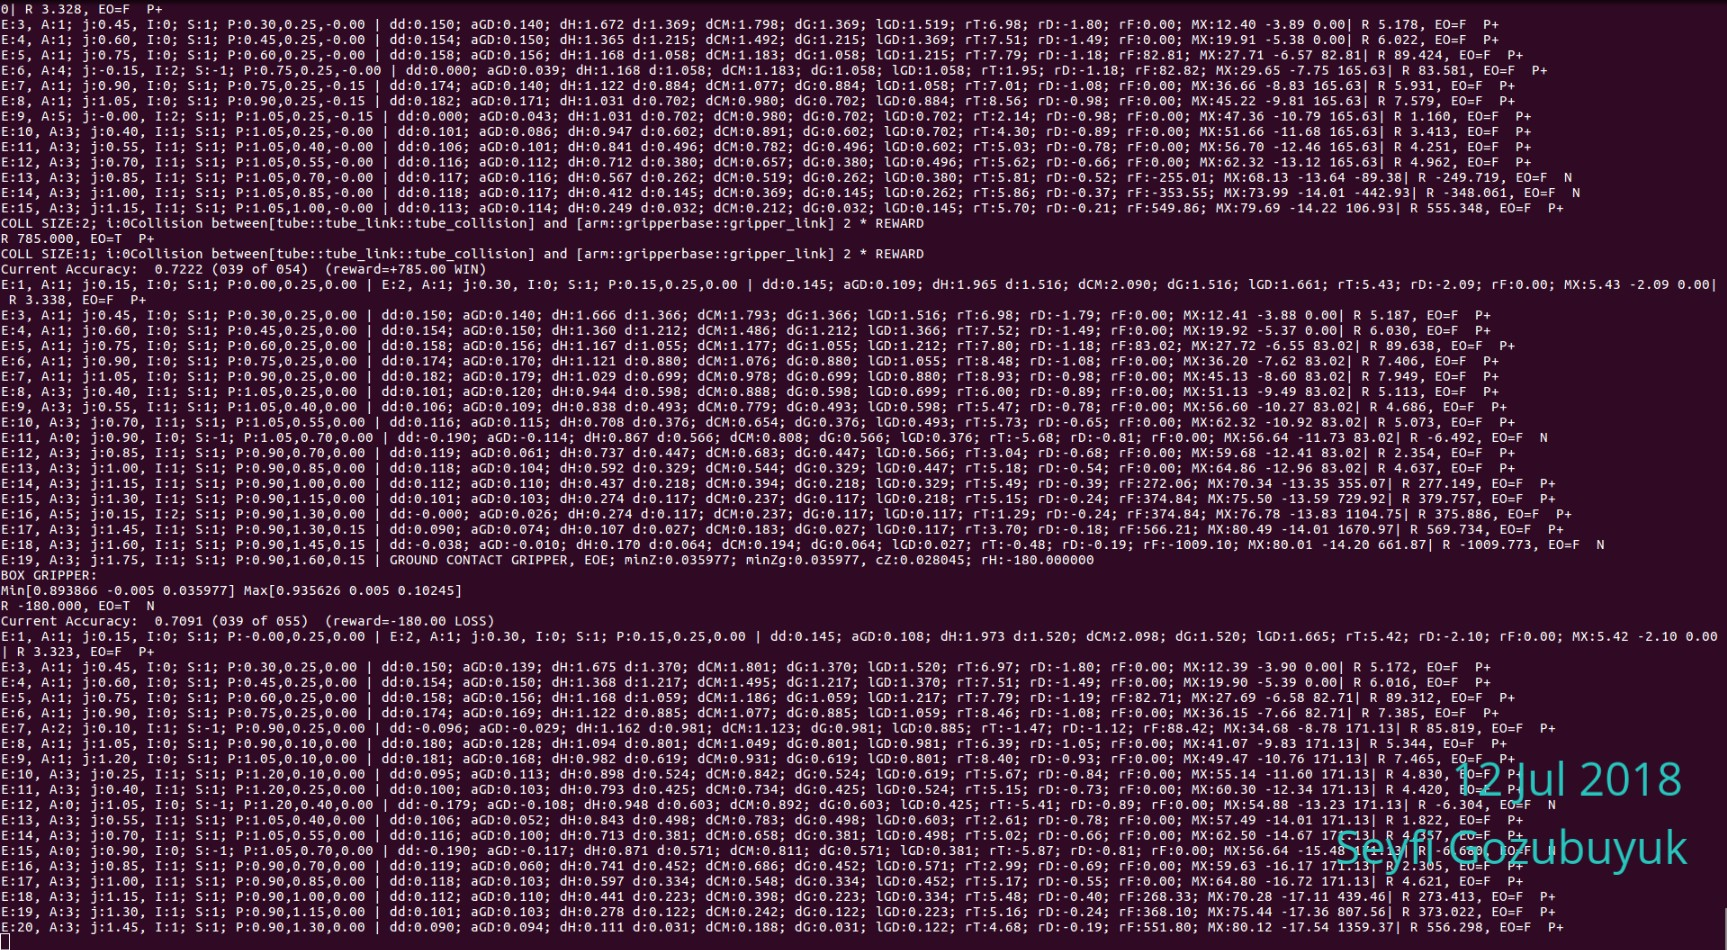
\includegraphics[width=\linewidth]{figures/Task2_Step55_2.png}
      \caption{Task 2 Episode 55 Console}
      \label{fig:t2s552}
\end{figure}

\begin{figure}[thpb]
      \centering
      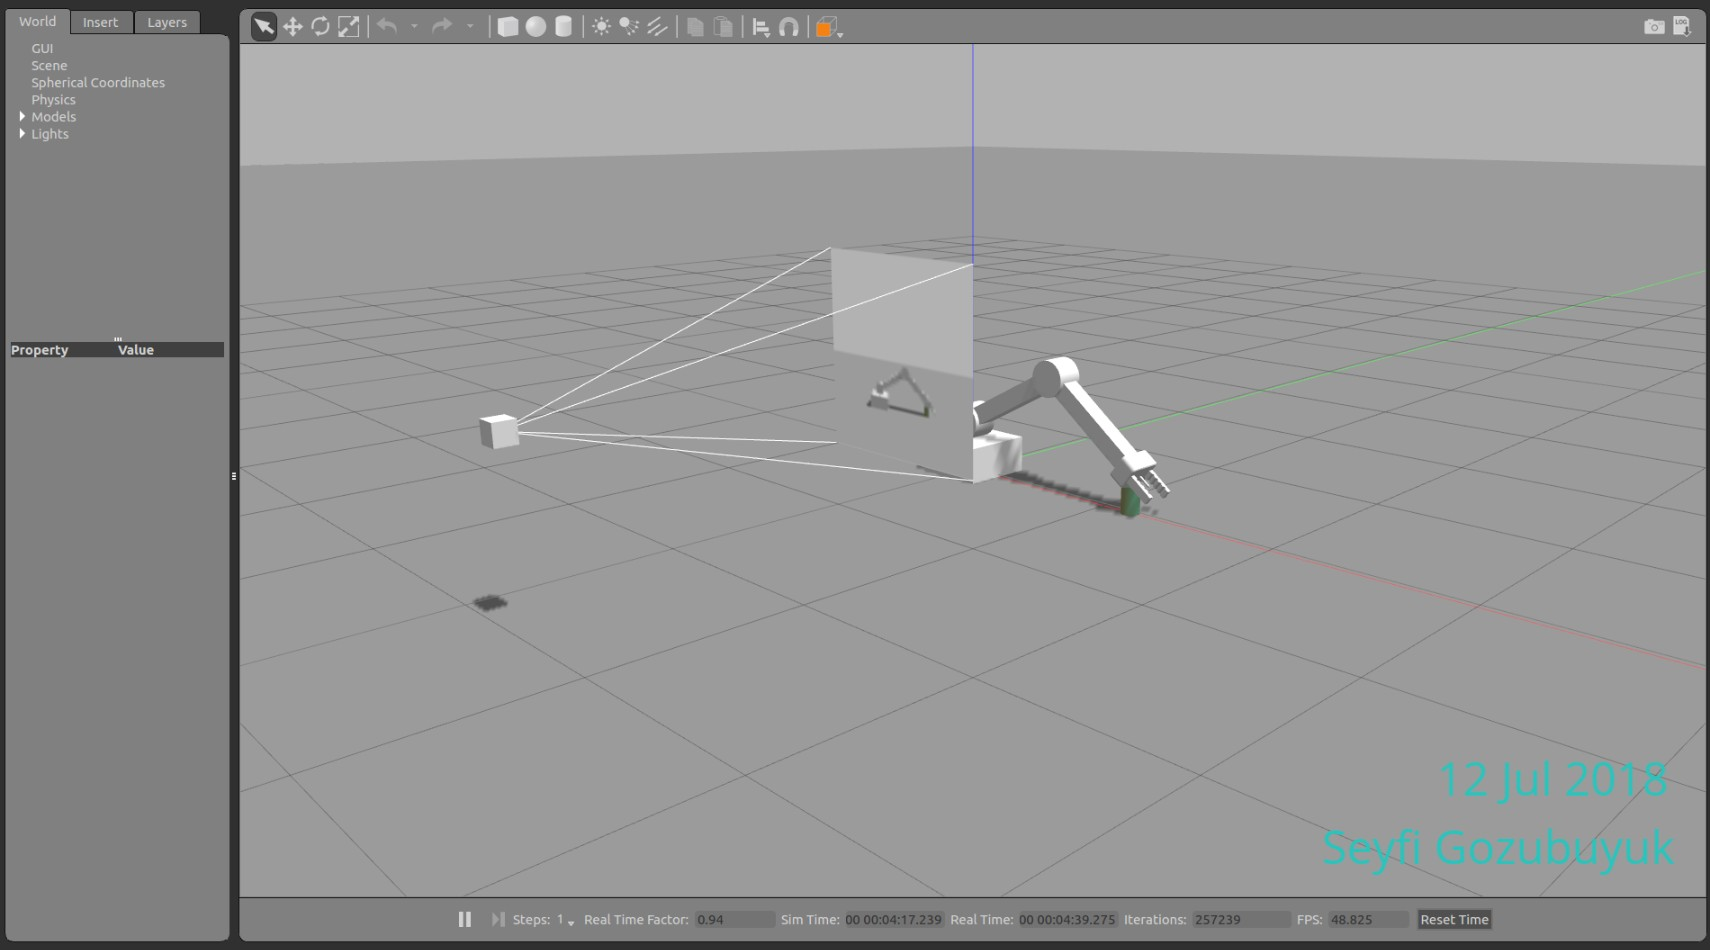
\includegraphics[width=\linewidth]{figures/Task2_Step94_1.png}
      \caption{Task 2 Episode 94 Gazebo}
      \label{fig:t2s941}
\end{figure}

\begin{figure}[thpb]
      \centering
      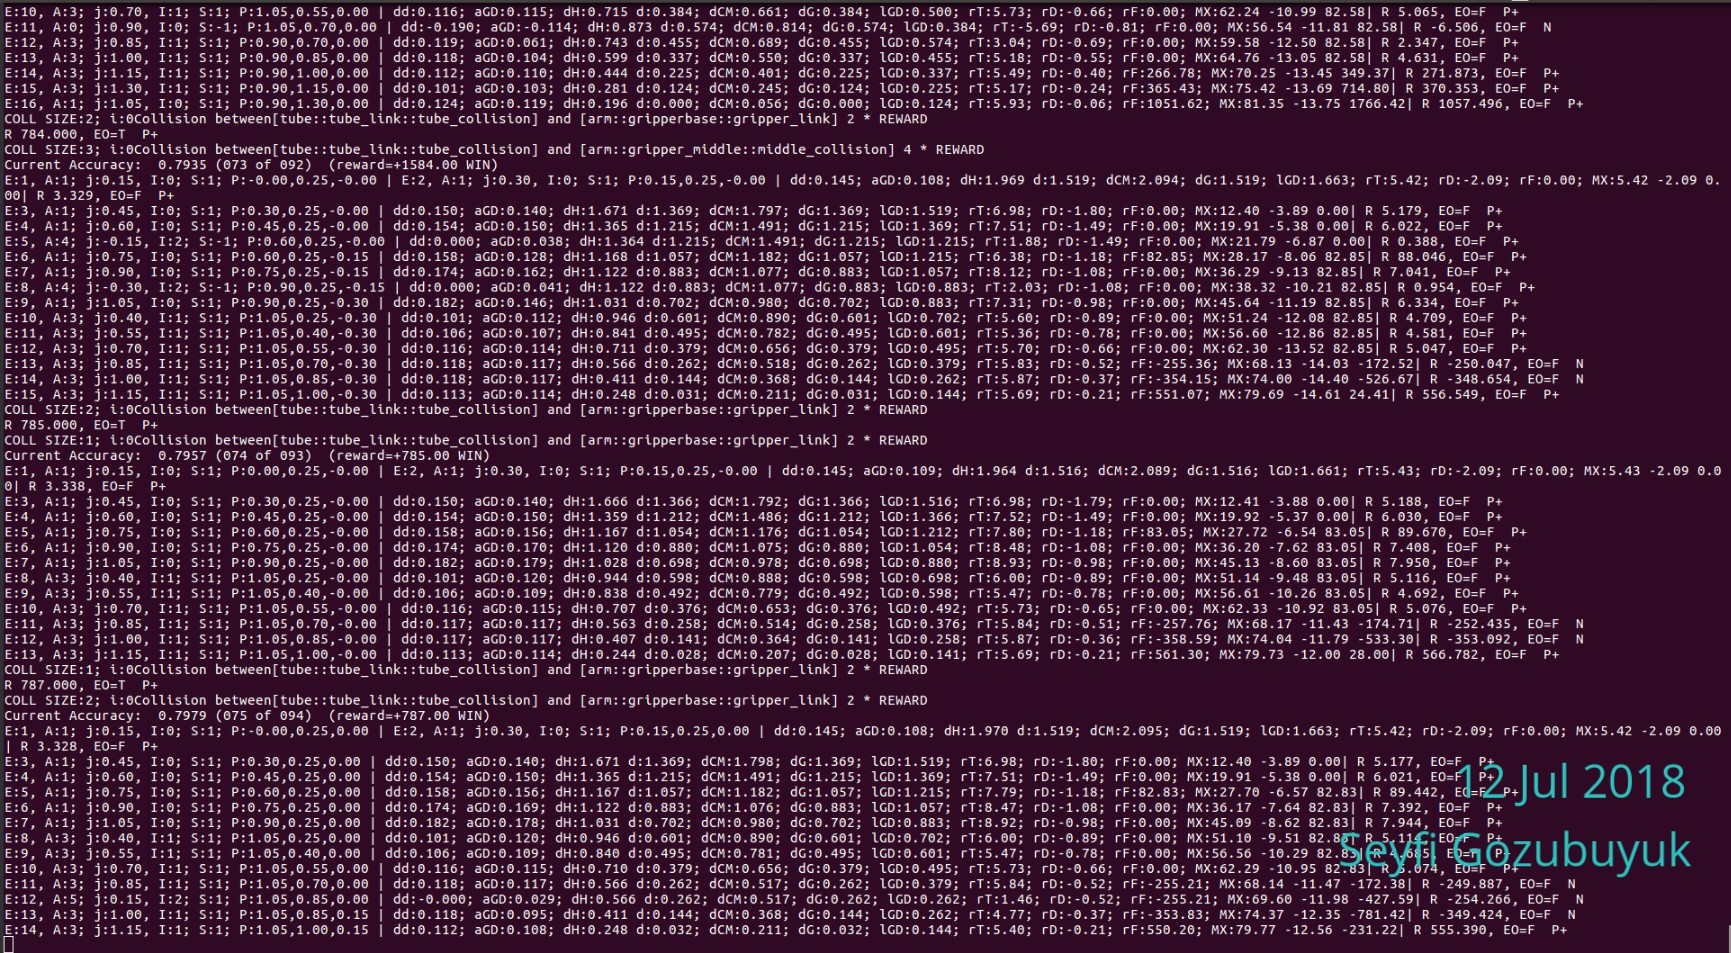
\includegraphics[width=\linewidth]{figures/Task2_Step94_2.png}
      \caption{Task 2 Episode 94 Console}
      \label{fig:t2s942}
\end{figure}

\begin{figure}[thpb]
      \centering
      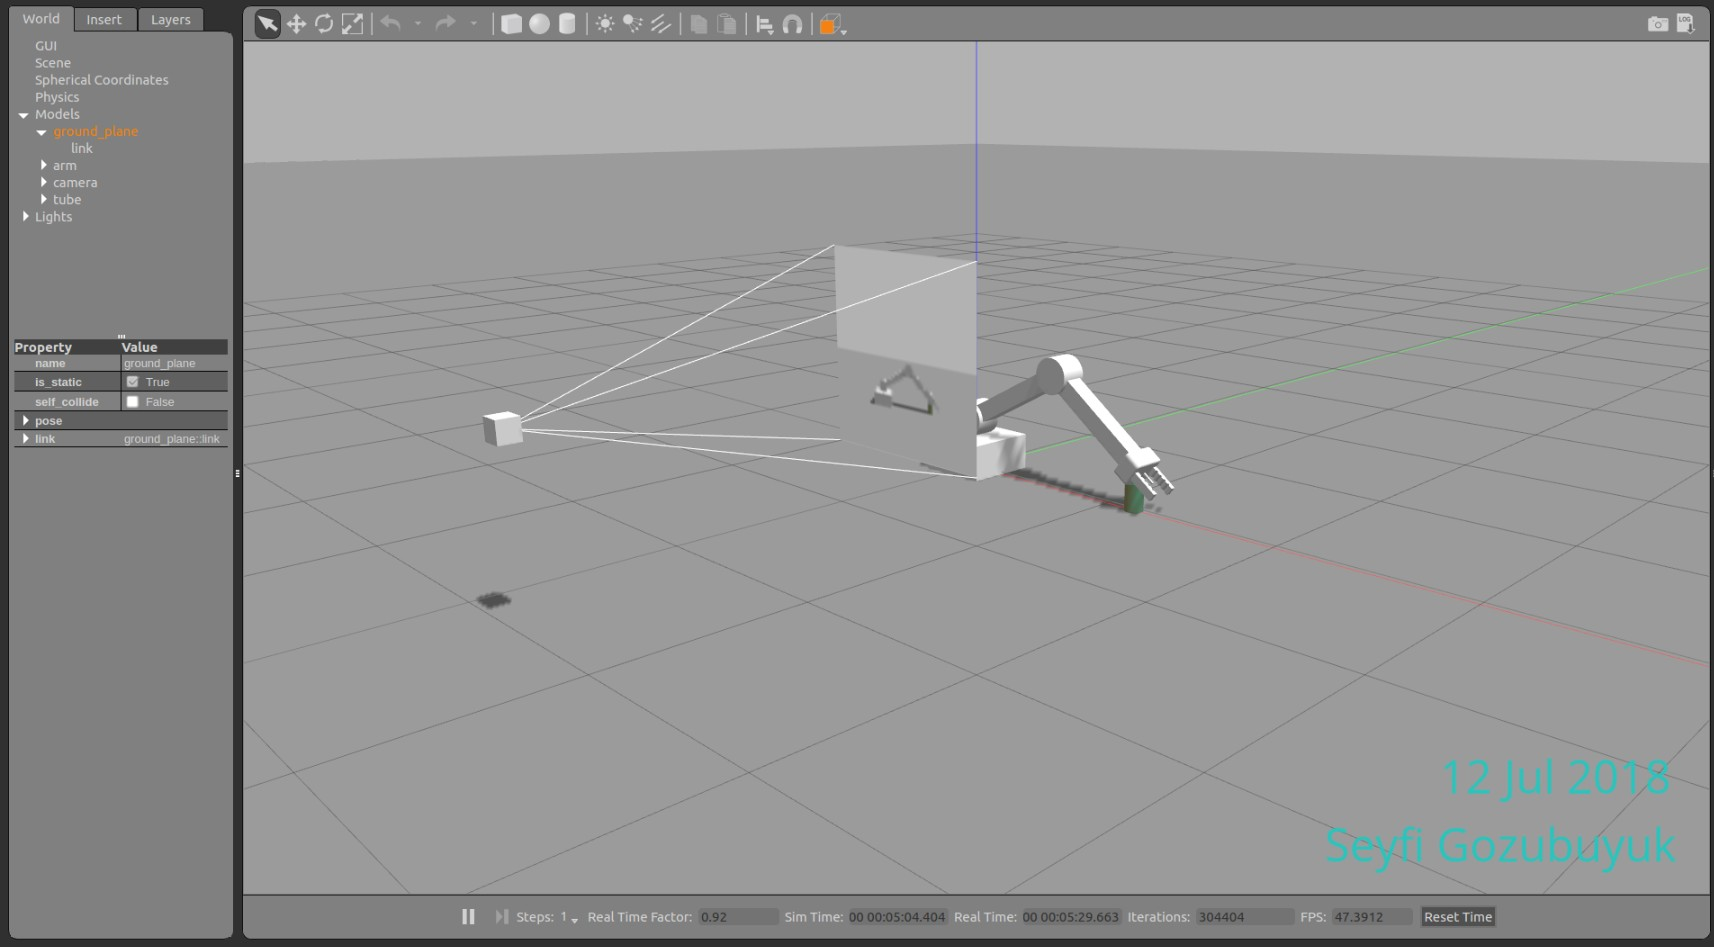
\includegraphics[width=\linewidth]{figures/Task2_Step113_1.png}
      \caption{Task 2 Episode 113 Gazebo}
      \label{fig:t2s1131}
\end{figure}

\begin{figure}[thpb]
      \centering
      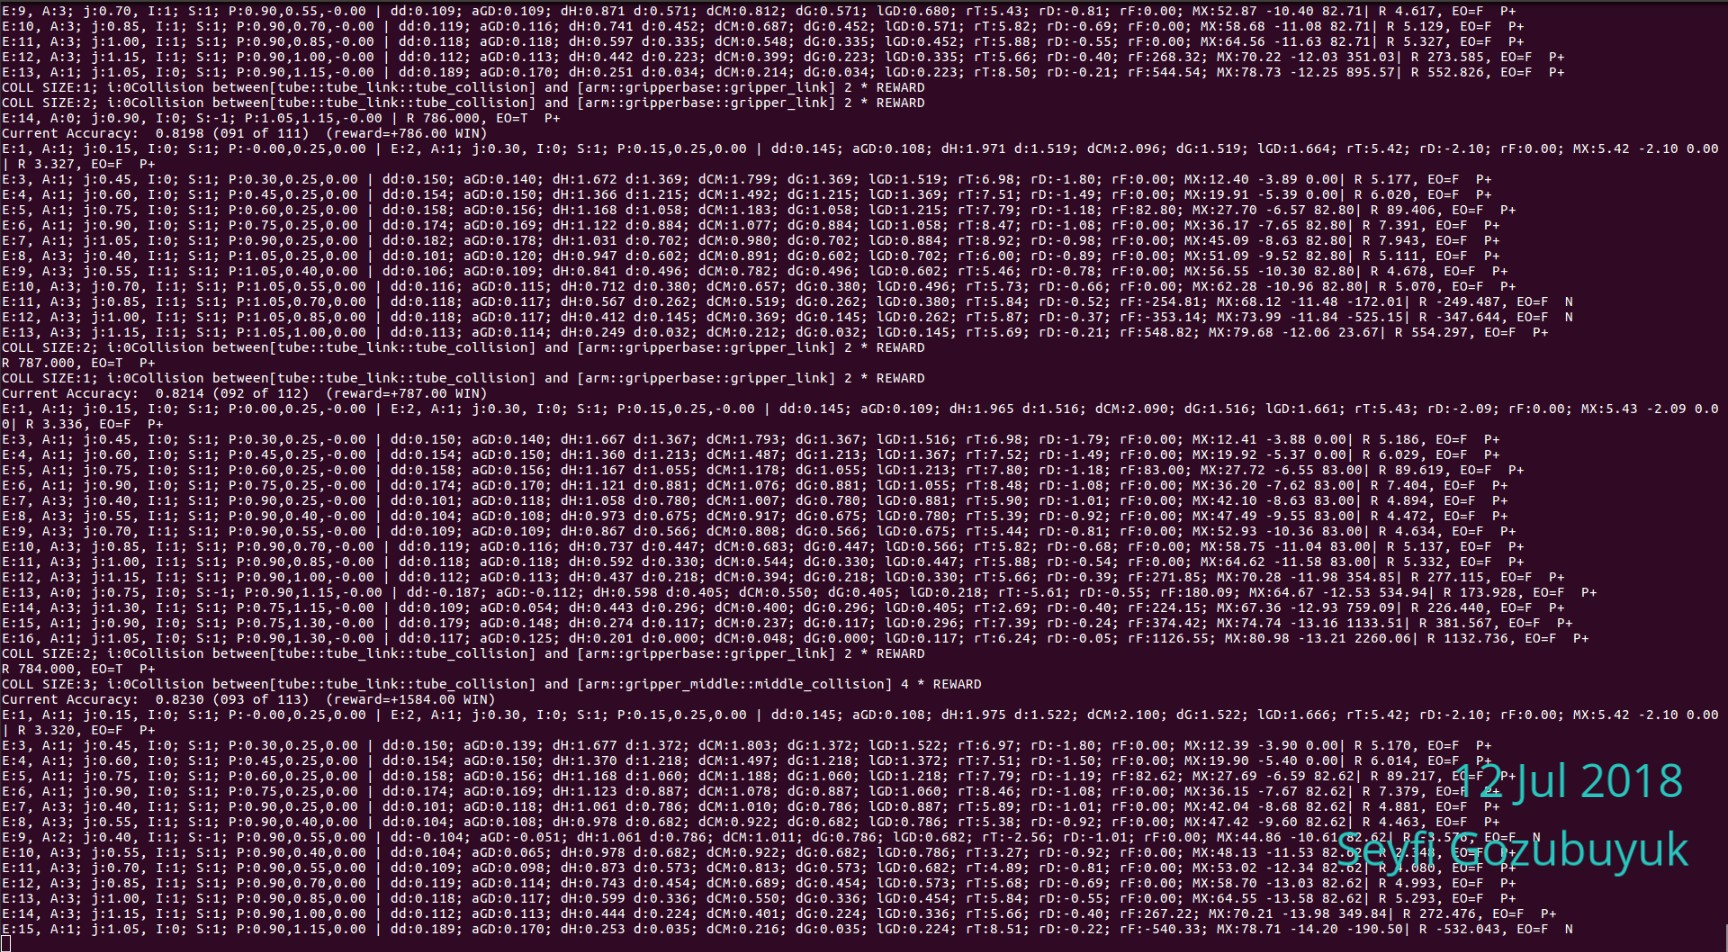
\includegraphics[width=\linewidth]{figures/Task2_Step113_2.png}
      \caption{Task 2 Episode 113 Console}
      \label{fig:t2s1132}
\end{figure}

\subsection{Technical Comparison} % only facts
The accuracy graph for both of the tasks are given in the Figures~\ref{fig:t1g},~\ref{fig:t2g}. Red line and points show the Reward value. For Task 2, the values are divided by 10 on the graph. The Yellow line and points show 100 for win and 0 for loss. Blue line shows the accuracy as the percentage value.
\begin{figure}[thpb]
      \centering
      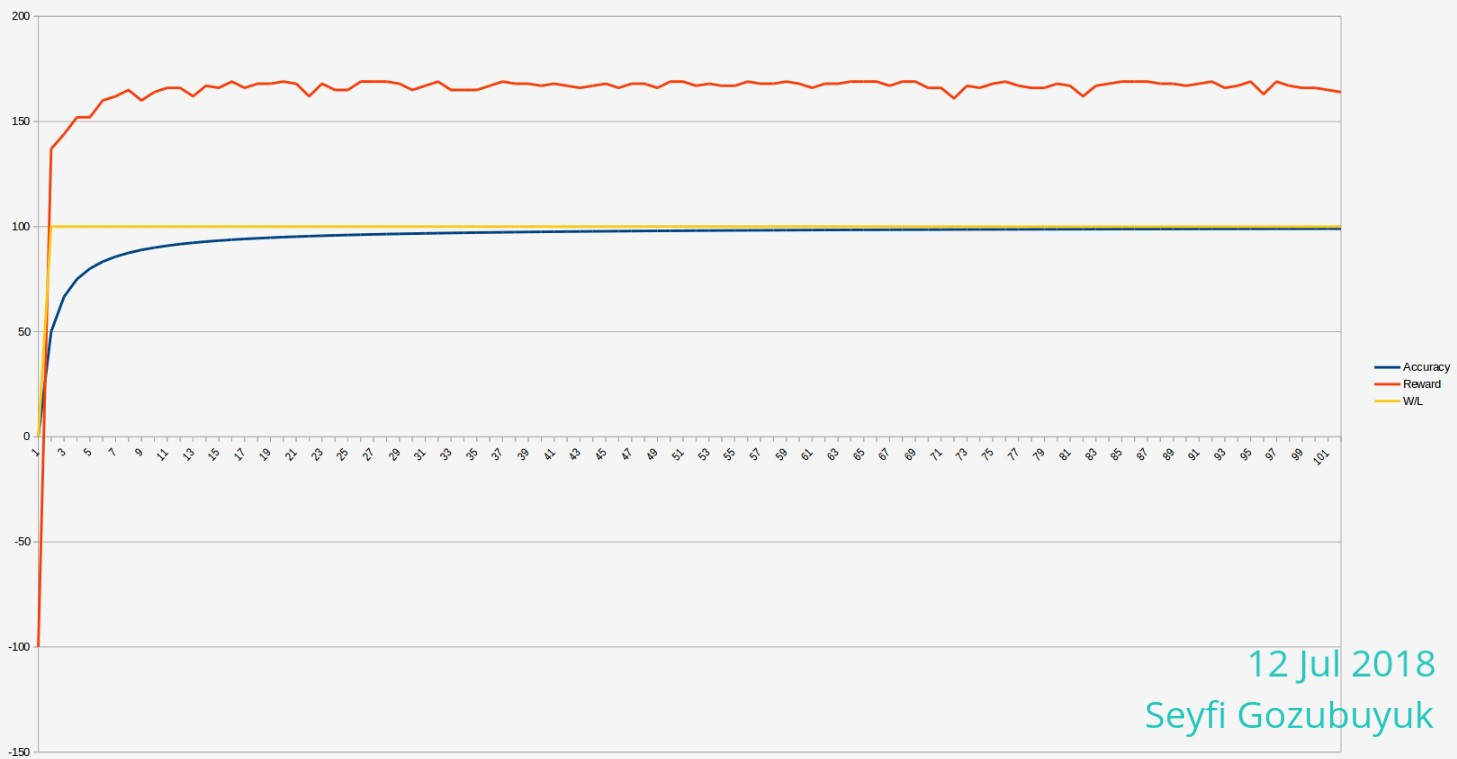
\includegraphics[width=\linewidth]{figures/Task1.png}
      \caption{Task 1 Result Graph}
      \label{fig:t1g}
\end{figure}

\begin{figure}[thpb]
      \centering
      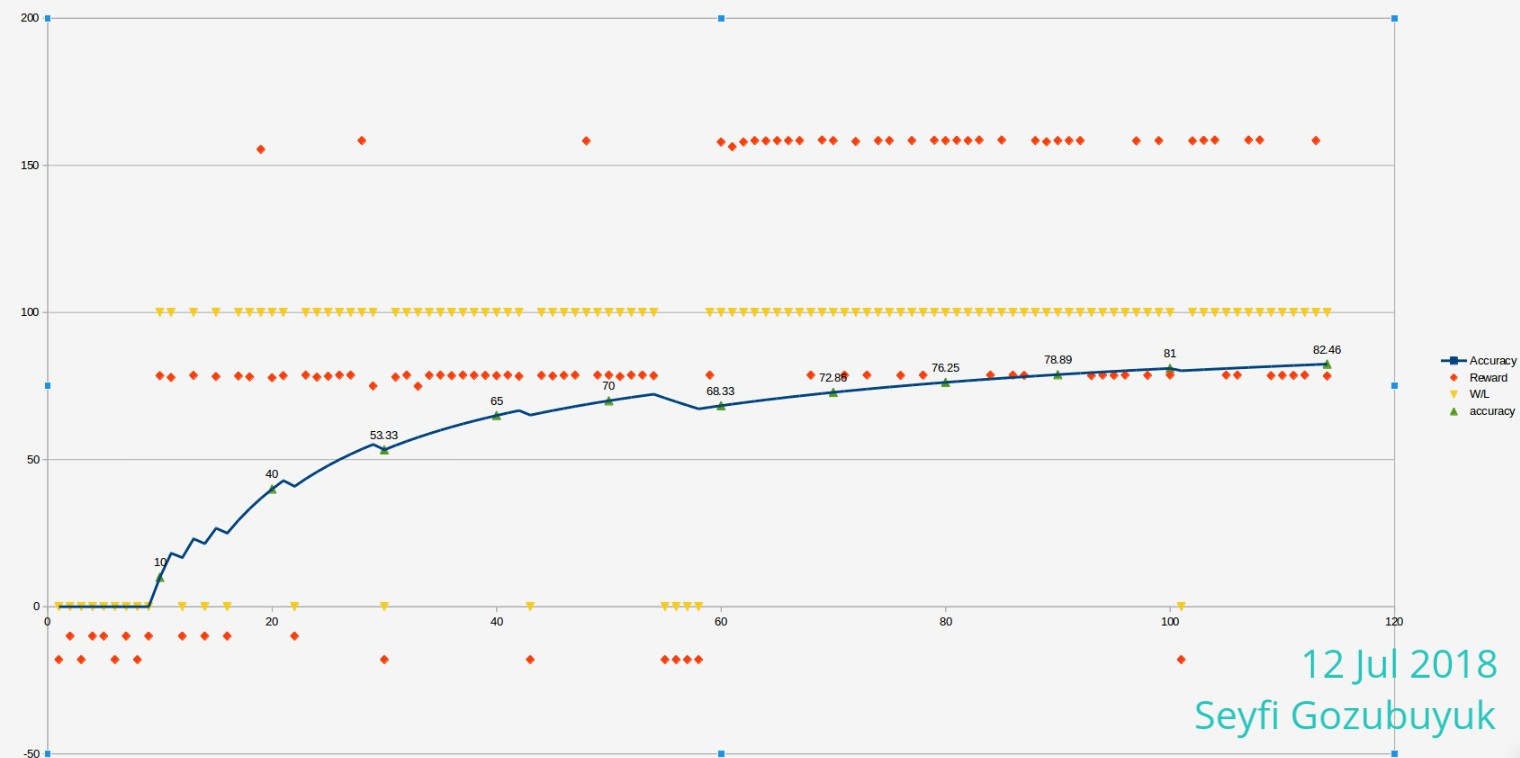
\includegraphics[width=\linewidth]{figures/Task2.png}
      \caption{Task 2 Result Graph}
      \label{fig:t2g}
\end{figure}

\section{Discussion}
The algorithm was able to teach the agent for the objective, and the robot arm was able to reach the object which was always in the same location.

Results: Explain the results obtained for both objectives. Include discussion on the DQN agent's performance for both objectives. Include watermarked images, or videos of your results.

Student should describe and briefly explain the results they achieved for both objectives. The discussion should also include their comments on the DQN agent's performance and if there were any shortcomings. Student should include either watermarked images of their results, or attach a video that displays the results and the arm in action.

Future Work: Briefly discuss how you can improve your current results.

Student should discuss on what approaches they could take to improve their results.

The algorithm was able to create a map for each environment. The robot navigated for almost two laps in both of the worlds. Both of the map images look warped. The parameters for the algorithm should be optimized, but due to time limitations, the tunning operation would be future work.

\section{Conclusion / Future work}
The parameters and the rewards can be improved. Besides, the algorithm may enable the robot to grasp the object. The agent should be trained to access objects that located randomly. First, only on the x-axis, then both on the x-axis and y-axis.\\
Testing the algorithm on the Jetson TX2 and comparing the results with the current results is a waiting task for the future work. Upon receiving successful results, the algorithms in the project can be used on a real robot

\subsection{Hardware Deployment}
The project was deployed in the simulation environment. The machine has an I7 CPU, 8GB RAM, and 650M GPU. The configuration was able to run the project, and with more powerful CPU and GPU, it will be possible to increase the complexity of the environment. Using a Jetson TX2 would enhance the performance of this project.

\bibliography{bib}
\bibliographystyle{ieeetr}

\end{document}